\documentclass[12pt]{article}
%title page stolen from J. Walton-Rivers with his permission :).
\usepackage{cite}
\usepackage{graphicx}
\graphicspath{ {./images/} }
\usepackage{IEEEtrantools}
\usepackage{float}
\usepackage{times}
\usepackage[british]{babel}
\selectlanguage{british}
\usepackage{pdfpages}

\newcommand{\game}[2]{\textit{#1}}{}

% debug lines
%\usepackage[showframe]{geometry}

% Shamelessly nicked from stackoverflow (JWR)
\usepackage{titling}
\renewcommand\maketitlehooka{\null\mbox{}\vfill}
\renewcommand\maketitlehookd{\vfill\null}

\title{CE913 Final Report: \game{Sticky Beaking}{}}
\author{Robert Marc James-Stroud, Vandana Sharma, Hao Wang, Su Zhang}


\begin{document}
	
% enable access to the 'special' variables
\makeatletter
\begin{titlepage}
\null\vspace{5cm}
		
\begin{center}
\begin{LARGE}
\textbf{\@title}
\end{LARGE}
			
% skip 2 lines
\vspace{2\baselineskip}
			
\begin{large}
\textbf{\@author}
\end{large}
			
\vspace{3cm}
			
Submitted as part of CE913, MSc Group Project.
			
% skip enouph to put supervisor at the end
\vfill
			
Supervisor: Dr. Jon Chamberlain\\
School of Computer Science and Electronic Engineering \\
University of Essex
			
\vspace{2\baselineskip}
			
\@date
\end{center}
		
\end{titlepage}
% disable access to the 'special' variables
\makeatother
\clearpage

% Rest of document here
\pagenumbering{roman}
\tableofcontents
\newpage
\newpage
\listoffigures
\newpage
\listoftables
\newpage
\pagenumbering{arabic}
\setlength{\parskip}{1em}
%do not touch anything above this line!
\section{Introduction} 
\game{Sticky Beaking,}, originally \game{Cluster Duck}{}, is a 2D casual puzzle game developed for PCs (Windows based platforms) and Android devices. The game revolves around the idea of `what home means to you'\cite{ggj19theme}, the theme for Global Game Jam 2019; from which \game{Sticky Beaking}{ } originates.   

\game{Sticky Beaking}{ } follows the trials and tribulations of a duck building a nest. Flying and walking around the a forest, the player must pick up twigs and return them safely to the nesting site. Failing obstacles results in the dropping and destruction of the twig.    

\subsection{Project Objectives}
The objective of this project was to create a game during the 2019 Global Game Jam Weekend which would act as foundation from which the team could build on post-GGJ with bug fixes, content and multi-platform support.         

\subsection{Methodology Employed}
Scripts for \game{Sticky Beaking}{ } are written in C\#. The reasons for choosing C\# are evident in the quote below and discussed in section \ref{unitylanguage}.

\begin{quotation}
\emph{C\# is a simple, modern, object-oriented, and type-safe programming language that combines the high productivity of rapid application development with the raw power of C and C++. Written by the language's architect and design members, C\# Programming Language is the definitive reference for C\#}. \cite{hejlsberg2003c}.  
\end{quotation}

Employing an agile approach for the development of \game{Stick Beaking}{ } was essential for success during the GGJ, as sprints were short; lasting minutes to a couple of hours maximum; waterfall's model was too rigid to allow the flexibility required to create, build and test without a fully formed requirements analysis. Development methodology of the agile model has been turning out have the capability to improve developing efficiency, It has the advantage of ensuring that the project adapts to the planning and current status of the development process and encourages developers to make changes as rapid and flexible as they can\cite{lee2010toward}\cite{dybaa2008empirical}.

\subsection{Hardware, Software and tools}

The game is created on PC platform mainly in Unity3D and Visual Studio 2017. Other software like Adobe Photoshop and Overture are used to create pictures, animations and background music. 

\section{System Design}
\subsection{Requirements}
This Requirement section is intended to be describe internal work as part of the 2019 Global Game Jam between team members building a game. It contain the software product specification and any constraints that need to be addressed. \cite{SRS}

\subsubsection{Overall Description}
Product Perspective: Cluster Duck as an interactive single player game that targets children. It was intended that development for Android and PC users would take place. The introduction of this SRS was based on the theme of the GGJ 2019. A game executable is provided for windows, Unity will handle these building processes.

Interfaces: There are numbers of interaction between user and software. The menus provided in \game{Sticky Beaking}{ } can toggle the game's sound effects ON or OFF. The volume of music can also be adjusted by the player. 

While in-game  the player can pause, restart or quit the game to main menu, and in main menu again there are options to `start game' and to quit the application. 

The player can connect directly to the game on a laptop or desktop machine via the keyboard and mouse.

Software Interfaces:\game{Sticky Beaking} is built in Unity software and it is a light weight application which sets the targeting of minimum operating systems. The game is built using Unity3D game engine as it can handle all aspects of game development.

User Characteristics constraints: Children of primary school age are the intended audience for the game \game{Sticky Beaking}{}. Children not attentive towards the written instructions in games therefore if game controls are complex or objective is unclear or ambiguous, they will quit playing. To resolve this issue instructions in the form of an image with clear, concise and simple language is needed.

As this game is for young audience, it will collect no personally identifiable information. No personally identifiable information is required to play either. Using only nicknames to record the high score in the game; nicknames are not consider to be personally identifiable information.

Apportioning of Requirements : The game is consist of database usage for competitive leader board. Game difficulty is set to make game more challenging and interesting. Animation is used to make movement interesting, static sprites will not entice play.

\subsubsection{Specific Requirements}
Programming Language: Game is built is Unity3D and scripts are written in C\#.

Target Platform: Game is developed to run on Windows 7 and above for PC based players and Android OS 4.1 if playing on a mobile-phone or tablet.

Player Input: The game can be played using correct input key and if correctly interact with the software using input keys.

Rotation of Player Character: Rotation of character is based on the direction given by the player using keys while game is active.

Collision Detection: The game will handle player - environment collisions predictably.

Sound Effects: Some sound effects like background music and collision of bird sound is added to the game to make it more informative.

Sprites: Sprites are used to make game interesting for the targeted audience, also used to direct players through the map.

Menu: The game has a fully functional menu with options that allow you to change control key binds and sound options, start game and quit game.

Score and Leader Board: Leader board is use to display the score of the game. As mentioned above that they are not connected to the server so scores are store on the local system in text file.

Map, Arena or Game World: The game area is designed for completion by as many players as possible, there should be good reason someone cannot complete a level (e.g. disability so they cannot control the duck properly).

Levels and Difficulty Settings: multi-level game with difficulty adjustment, currently game is of a single level with static difficulty.

Language Options: The game is built in one language only.

Animation: The game could have more clear and detailed animation covering several aspects like flying and walking.

\subsubsection{External Interfaces}
Keyboard and mouse: For windows platform we have mouse and keyboard to control the payer character.

Leader board: It is an interface with a database for output the score in it.

Functions: System is designed to ignore all other inputs that do not match control. Unity is the engine designed to handle mostly abnormal situations and try to recover.

Software system attributes: There is no issue of security in this game as game is not using any user-name or passwords that need encrypting, game is using database to store and display on the leader board and there is no use of server, data is stored locally on the system.

\subsection{Component level relationship}

According to Bartle in \cite{funandgameplay}, games can be described in terms of their tokens, rules, features and dressing. In this instance, however it only serves to be interested in the first two of these when describing the component level relationship in \game{Sticky Beaking}; tokens and rules, as gameplay is an emergent property of the two.

Tokens are gameplay significant objects - most commonly, nouns. Rules describe what you can do to tokens - these are verbs. Features and dressing do not carry much weight in describing a component level relationship.

In computer games, tokens are usually the programming objects that will have associated assets and properties whereas rules refer to tokens and each other \cite{funandgameplay}. 
\begin{table}[H]
\centering
\begin{tabular}{| p{6cm} | p{6cm} |}
  \hline
     \bf Duck collide with Other Tokens  & \bf Rules\\ \hline
     Ground, Tiles and rocks & Duck collide with these tokens and reset flight time. \\ \hline
    Trees & When Duck collide with these tokens and reset flight time and need to fly over the tree as they are colliders. \\ \hline
    Vorago & On collision with duck or when duck falling in it, lose the twigs collected by them as penalty.  \\ \hline
    Cactus & They are just collider in the game colliding with the duck.  \\ \hline
    Fences & Collider act as boundary in the game  to restrict duck or player movement in the game arena.  \\ \hline
    Owls & They are the NPC in the game, if player token collides with Owl token it become uncontrollable and lose stick if carrying one.  \\ \hline
    Twigs & Player can collect twigs on collision with twig token but only one at a time .  \\ \hline
    Nest & If player is carrying twig token and successfully collide with Nest token then Nest build will increase by one step.  \\ \hline
    Cactus & They are just collider in the game colliding with the duck.  \\ \hline
\end{tabular}
\caption{Component level relationship table for \game{Sticky Beaking}{}}
\label{tab:comprelationship}
\end{table}

\subsection{Game Design}

This section of report is about the game design of \game{Sticky Beaking}{}. It includes detailed descriptions of the design decisions and justifications for the decisions for the main components of the game.

\subsubsection{Targeted Audience }
The game is specifically designed for young children or children of primary school age. Most children today classify as `digital natives' \cite{helsper} growing up with technology and the internet, with an interest in playing games on these devices. 

\subsubsection{Description}
\game{Sticky Beaking{ }} is single player game developed for Windows 7 and above platforms as mentioned previously. While playing the, intent of the player is to gather twigs from the surroundings and build a nest for the duck. Twigs spawn in the environment in an unpredictable manner, causing the game to be different each playthrough. The nesting site is fixed position represented by a sprite to make it easy for the player to search it. While playing, the player will interact with different objects in the environment. These interactions will act according to the rules defined in table \ref{tab:comprelationship}.

\subsubsection{Idea and Story}
As mentioned above in the report that game is designed during the Global Game Jam 2019 based on the theme `What Home means to you' \cite{ggj19theme}. Multiple different ideas and concepts were floated, debated and rejected before settling on the original idea for \game{Cluster Duck}. A few of these initial ideas are: defending your home from enemies, re-building a house the house with a time limit, collecting objects to complete the house, Collecting food for the house and many more. 

After three hours of brainstorming and discussing it was realised that the idea for what 'home means to you'\cite{ggj19theme} was the freedom to feel safe; a common thread through all the ideas suggested. \game{Cluster Duck} was the result of this discussion. Although the title of `Cluster Duck' was used publicly during the GGJ, and therefore uploaded to the 2019 entries as such; it was suggested that this name might not be appropriate for the ages of the intended audience due to its similar one letter difference to a vulgar slang term of US origin. \game{Cluster Duck} was renamed \game{Sticky Beaking} with a unanimous team vote.

\game{Sticky Beaking}{} is the story of a duck who needs to explore the world for twigs to enable the construction of her nest. However, the world is dangerous and filled with obstacles. Flying around is also tiring so she must regularly land or will exhaust herself and fall to the ground. The challenges do not end when a twig is located, she has to safely return the twig to her nesting site, past the owls and chasms which still destroy the stick should she end up in them. Should she successfully return the twig to her nest it will magically grow a stage. 

\subsubsection{Aesthetics}
The game is designed in 2D and with assets of a colourful and simple graphical design, cartoon in nature. Colourful graphics are used make game more appealing to the targeted audience. 2D graphics are significantly cheaper when compared with 3D in terms of time to create (modelling, UVW unwrapping and creating the maps and textures) and the space needed to store all the required assets. 

Using 2D assets over 3D makes \game{Sticky Beaking}{ }mobile friendly, it also means that phones, tablets and lower specification machines could be supported as \game{Sticky Beaking}{ } has no dependency on having a dedicated GPU.

There was and early discussion for making 2D game in perspective instead of orthographic which would have given a more interesting effect when traversing the level as the background would not have appeared to be so static (see figure \ref{fig:orhtovspers} for orthographic vs perspective camera views in Unity3D). However this would have taken a full rebuild of the level, time that could have been better spent elsewhere so was decided against, leading to a game that is figure \ref{fig:orhto}.

\begin{figure}[H]
    \centering
    
\includegraphics[scale=0.2]{orthovsperps.png}
    \caption{Orthographic (left of the image) vs perspective (polygon on the right of the image) cameras in Unity 3D.}
    \label{fig:orhtovspers}
\end{figure}


\begin{figure}[H]
    \centering
    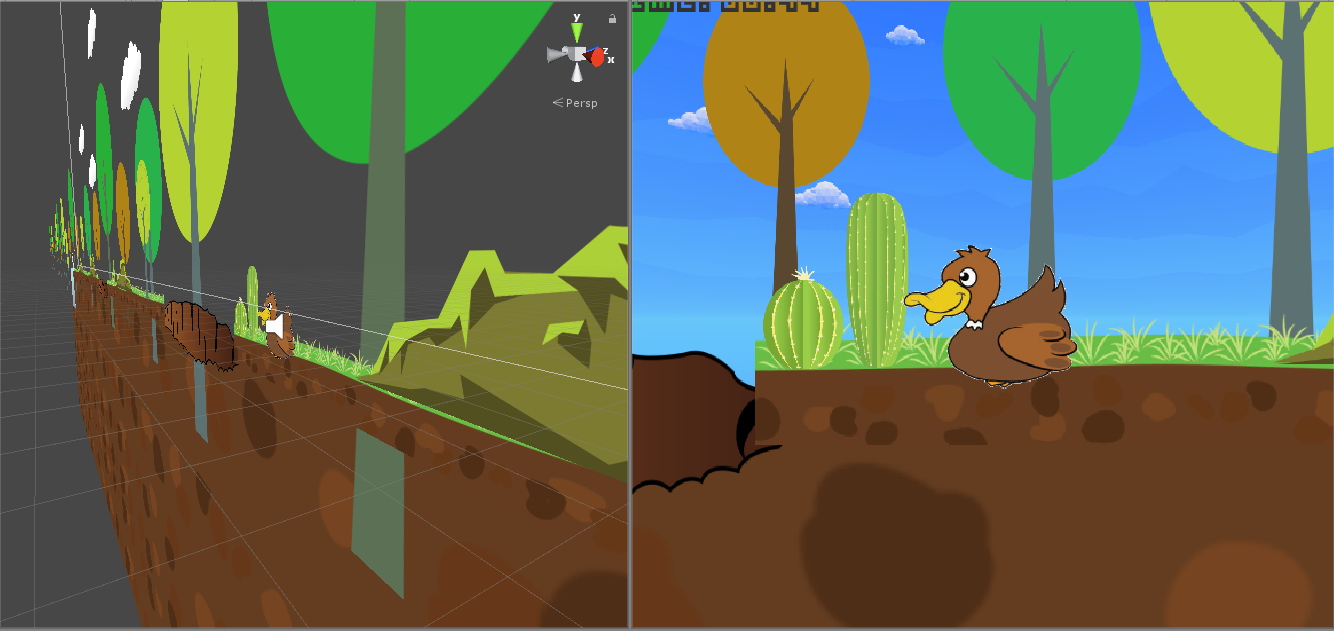
\includegraphics[scale=0.4]{ortho.png}
    \caption{An image showing the orthographic nature of \game{Sticky Beaking}{}. Left the positioning of the tokens and assets; right the game view showing no relationship between distance and object size.}
    \label{fig:orhto}
\end{figure}

\subsubsection{Characters}
\game{Sticky Beaking}{ } has a single main character, the duck, and multiple antagonists, the owls. Player character’s movement is controlled through the keyboard or mouse. 

\begin{figure}[H]
    \centering
    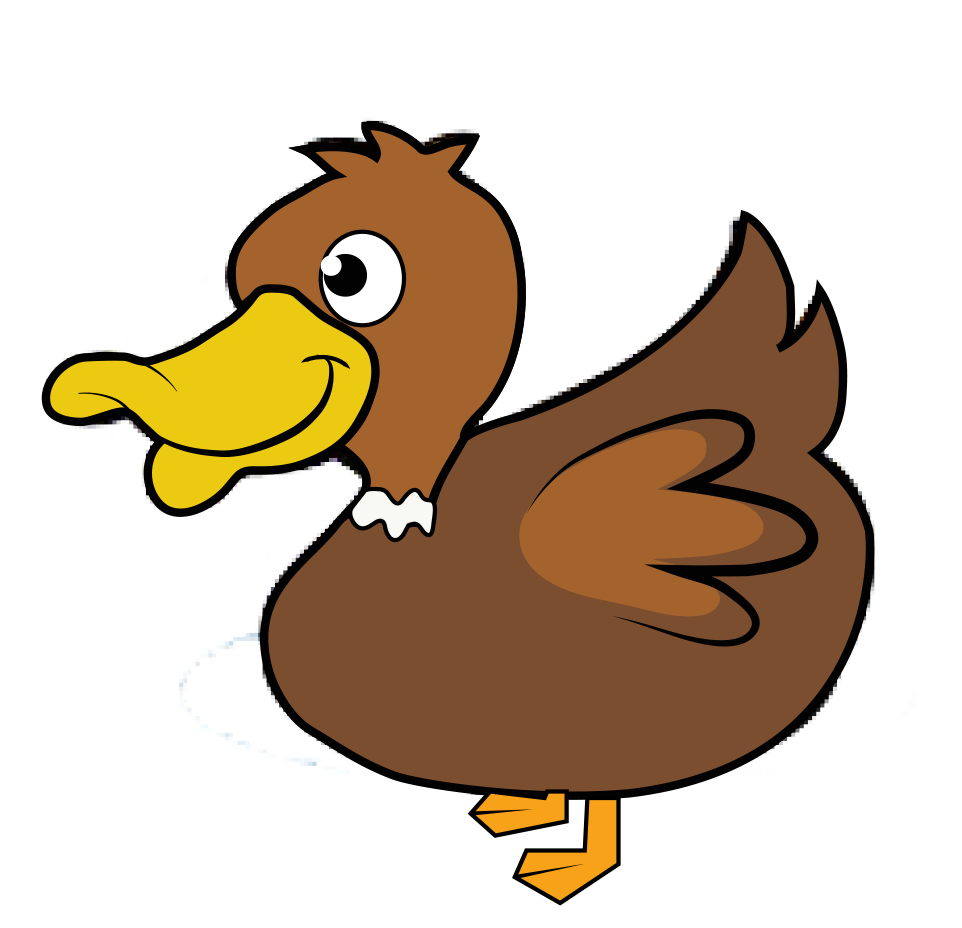
\includegraphics{duck.png}
    \caption{"Duck" the player character in the game}
    \label{fig:Duck}
\end{figure}

\begin{figure}[H]
    \centering
    
\includegraphics[scale=0.7]{owl.png}
    \caption{"Owl" the Non- playing character of game}
    \label{fig:Owl}
\end{figure}


\subsubsection{Level Description}

There is only one at present in-game. The level of the game is split into two parts connected with some tiles in the environment. The level is consist of graphical representation of rocks, some collider trees, plants and some enemies. 

\begin{figure}[H]
\centering
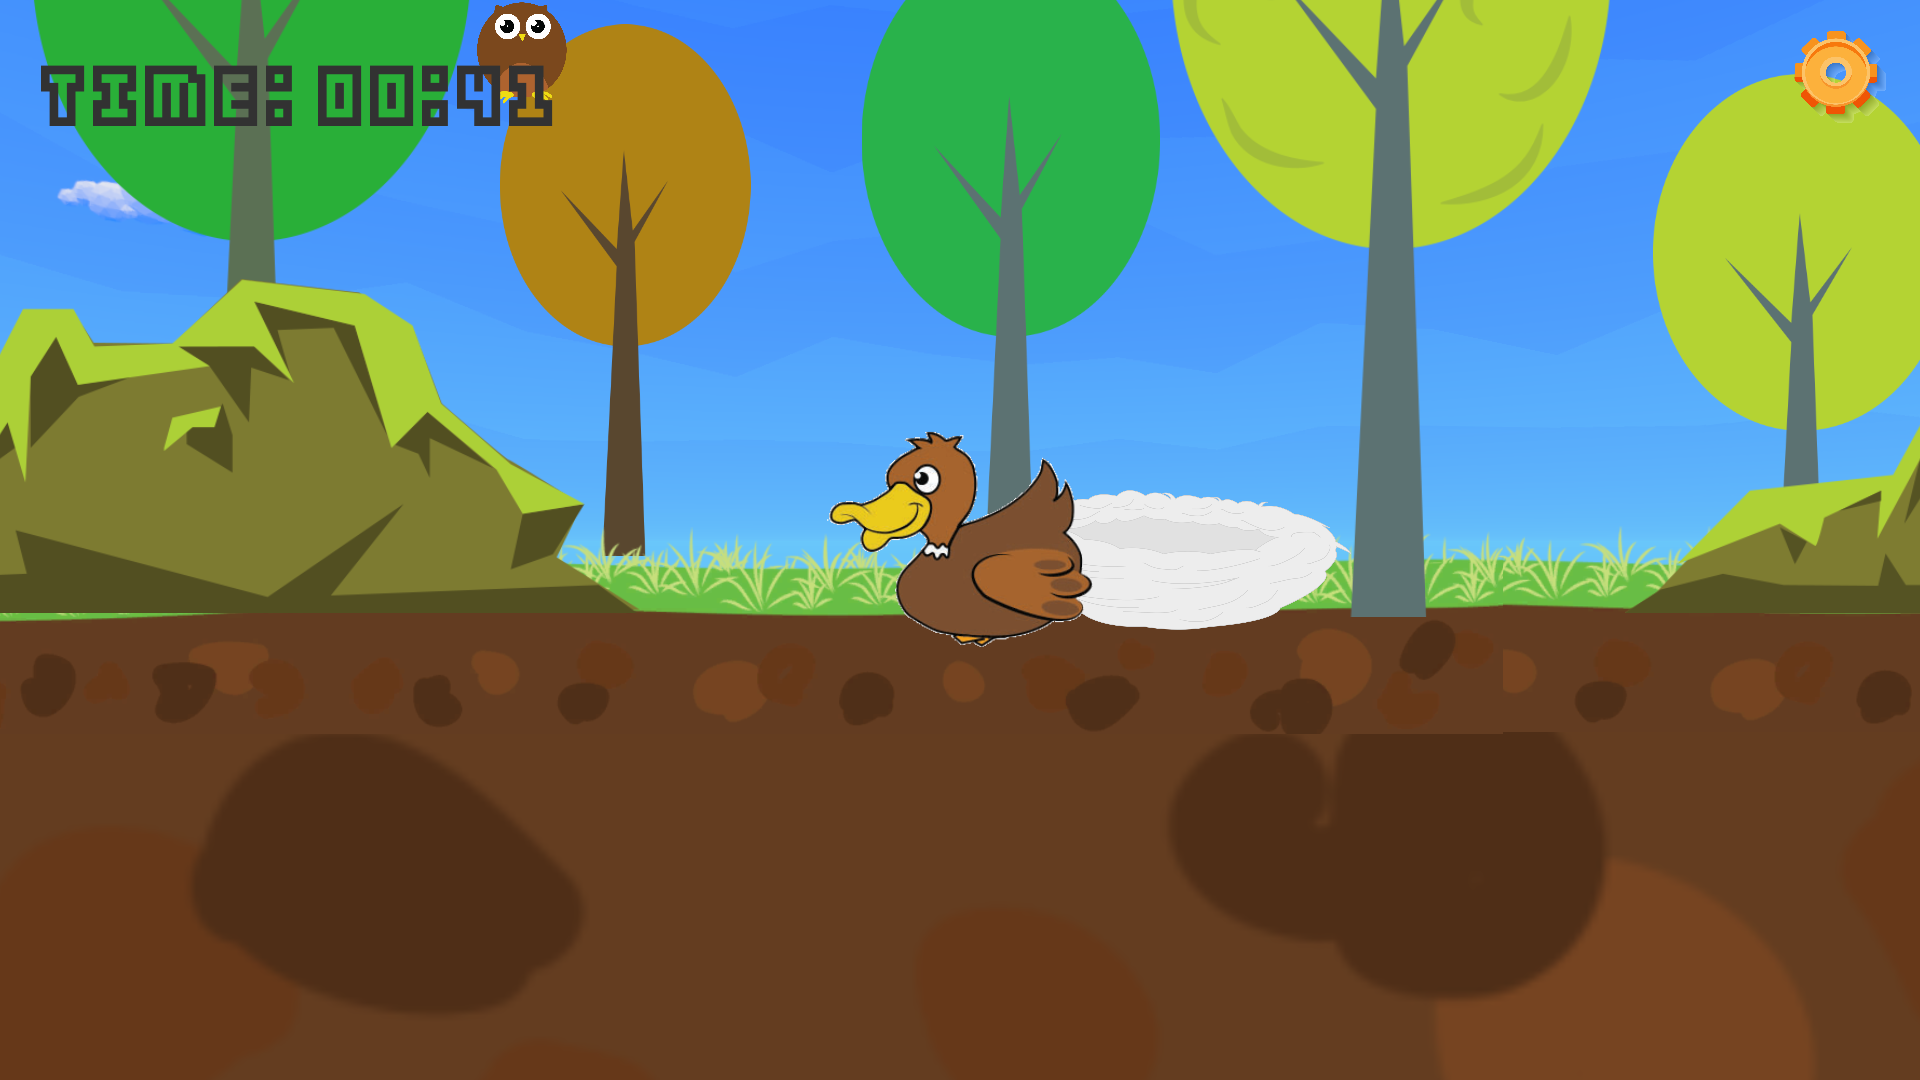
\includegraphics[scale=0.17]{level.png}
\caption{Level description of the game}
\label{leveldescription}
\end{figure}

\begin{figure}[H]
\centering
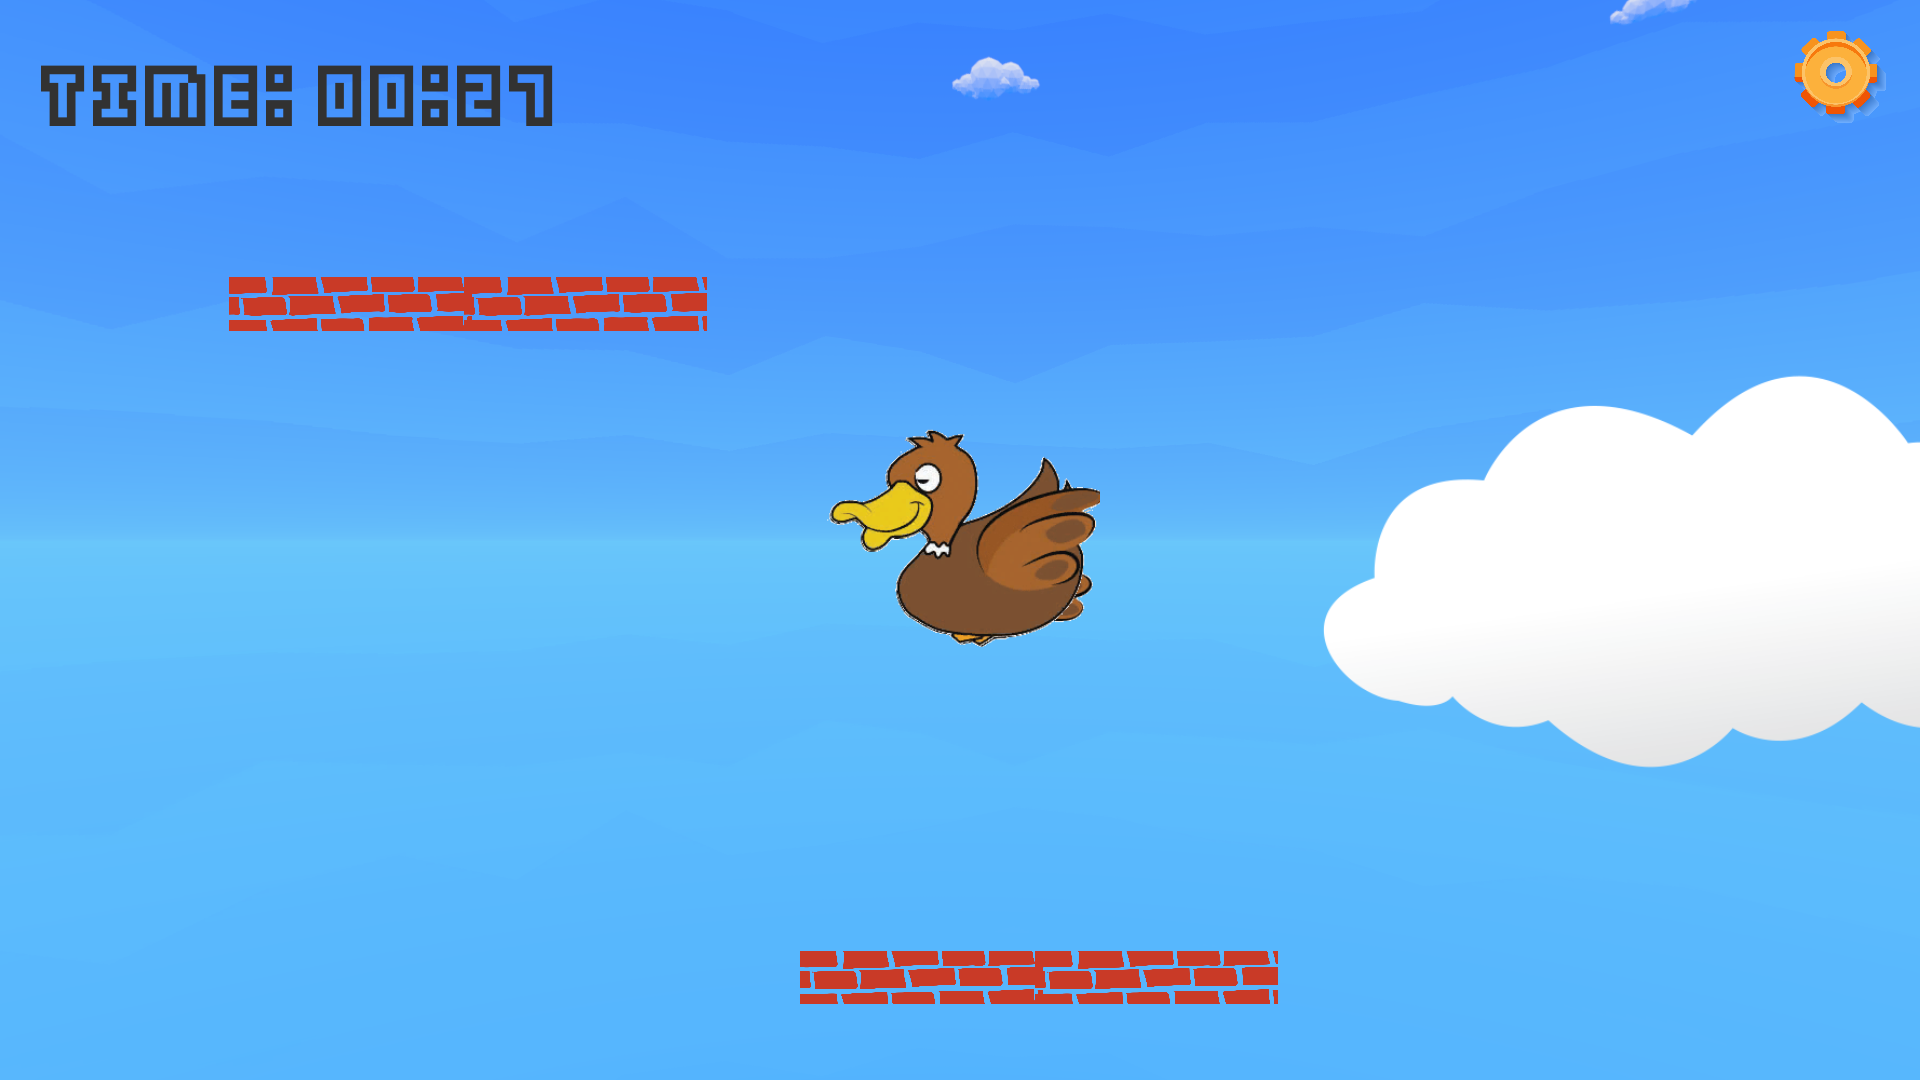
\includegraphics[scale=0.17]{tiles.png}
\caption{Tiles used to connect level map}
\label{tiles}
\end{figure}

\subsubsection{Graphical User Interface}
 
 Graphical User Interface (GUI) is one of the important part of game design. The use of User Interface is to make interaction between user and software simple as possible. We have used many GUI in the game like different buttons, texts, scroll bar and images.
 
 Menu: We have Menu in the game, designed with GUI buttons and texts. They are used by players to switch from one scent to other.
 we have \textbf {Start} button in main menu to start the game.
 \textbf{LeaderBoard} button to switch to leaderboard scene where we have all previous score saved. \textbf{Option} button intent to open option menu for the player and \textbf{Exit} to quit the game.
 
 Option: It is also a menu for user interface linked from main menu and this contains buttons like \textbf{PauseMusic}, \textbf{scrollbar} to control the volume of music and one \textbf{Back} button to move back to the main menu.
 
 LeaderBoard: This section is used to display score of the game and consist of texts and button. Text we used to display Rand, name and the time taking by the user and \textbf{Back} button to move to previous scene in the game.
 
 Start: \textbf{Start} button is used by user to start the game by switching to game scene.
 
 Setting button: This button is intent to display more available setting options for the user while playing the game. As we click on the this button it pause the game.
 
 Resume: This button is used to resume to the paused game to continue the game.
 
 Restart: We can restart the game using this button. This help user to restart game from the same scene.
 
 Time: \textbf{Time} is used to display the time duration of game and this is also used to calculate score at the end of the game complete.
 
\subsubsection{Game Controls}

Since this game is a PC game,it only supports mouse and keyboard controls. As it is also displayed in the game instructions that user can use only WAD keys. 'W' key is used to make duck fly, 'A' is used to make duck move in the left direction, 'D' is used to flip into right direction and similarly 'S' could be used tp move downwards to the ground, however this functionality is not present. Mouse click can also be used to make duck fly in the game.


\subsubsection{Scoring System}

Scoring system is important in the game to display the result of game and allow competitive play.

\game{Sticky Beaking}{ } uses \textbf{Time} as a scoring method. At the end of the game the difference in times are calculated from the starting time to the finishing time. The time taken by players to complete the nest build is in seconds as the time variable is cumulative using \emph{Time.deltaTime} (a unity method which returns the lapsed time between frames) and display it on the leader board. The leader board is displayed to the player in a numerically ascending order based on time taken to build the nest.

\subsubsection{Features, Mechanics and Gameplay}
Features

The main feature of the game is to create a casual game for children to play.Thus,it should have a quick start and the level isn't hard for them. Textures and pictures are designed as cartoon style to attract children.  

Gameplay

\begin{itemize}
\item Learning: The time players spent on understanding and dominating the game is short. There is a cartoon picture tutorial at the beginning of the game to show the player of the game system and mechanism. It is better to teach the novice by this way is mainly because players are more likely to be children. 
\item Motivation: Players can spend their free time to challenge themselves for shorter time to complete the game.
\item Emotion:The games can provoke players feel the fun and thinking about the strategies to achieve goals. 

\end{itemize}


\subsubsection{UML Diagram for design}

\begin{figure}[H]
    \centering
    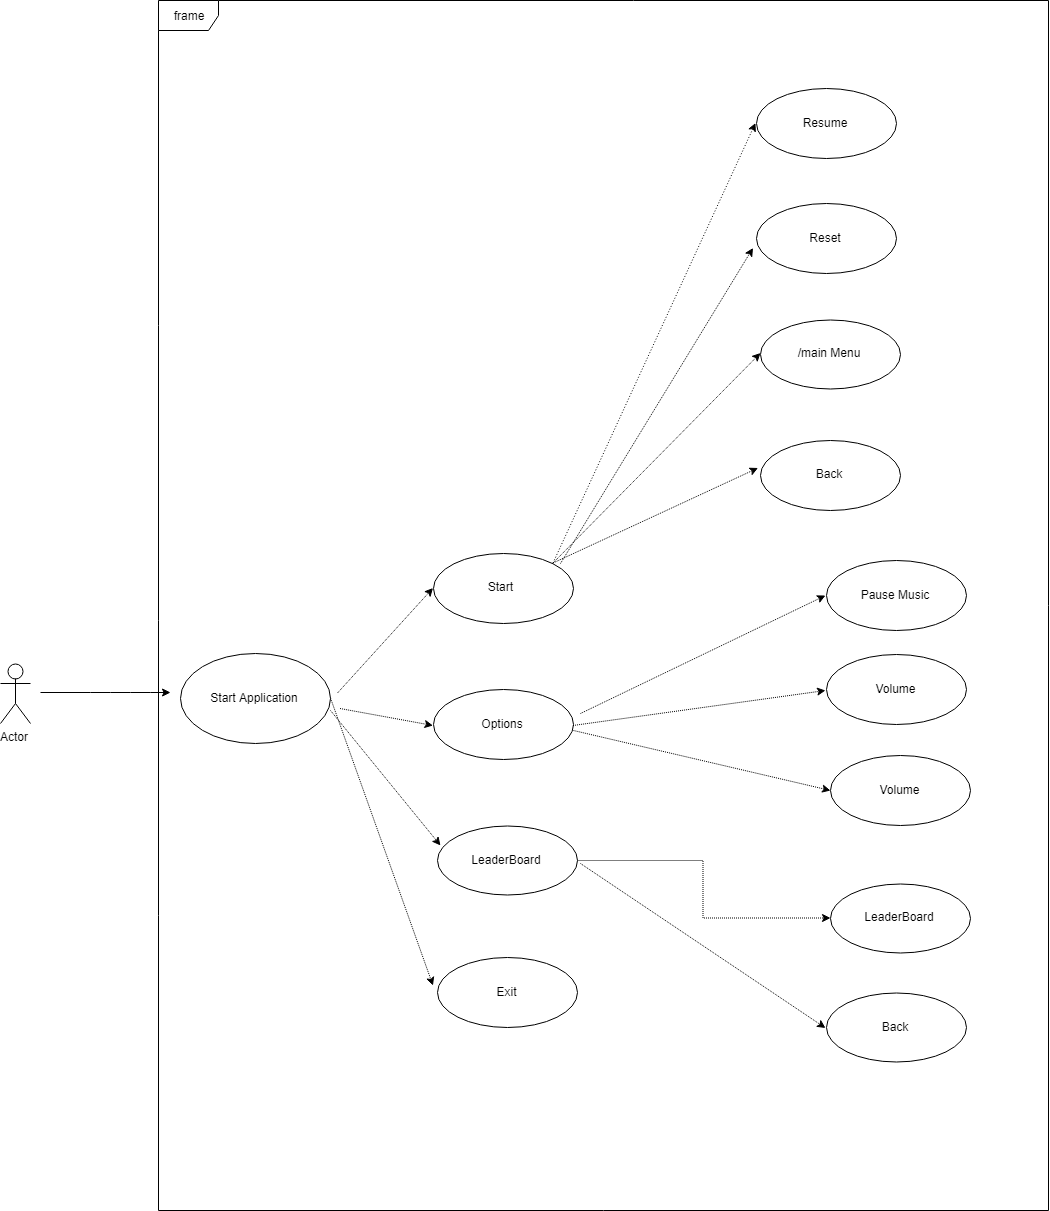
\includegraphics[scale=0.4]{UML.png}
    \caption{UML diagram for Game design}
    \label{fig:UML}
\end{figure}

\section{Implementation}

\subsection{Programming Language} \label{unitylanguage}
Unity provides support for C\# and UnityScript (a kind of Java Script), however most of the programming in games utilising Unity3D are created with C\# (see figure \ref{fig:piechart}), in 2014 80\% of projects were written in C\# \cite{unityblog}. As Unity primarily support C\# in the 2018 version of Unity3D \cite{unityprogramming}, the zealous nature of Unity's adoption of C\# across the board; with the volume of resources available online through Unity forums and Stackoverlow made C\# an ideal language. It is versatile and well supported.it made little sense to use any other programming language. Since 2014 in-house tutorials are written in C\# before being converted into UnityScript \cite{unityblog}. 

\begin{figure}[H]
\centering
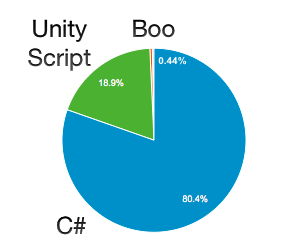
\includegraphics{graph3.png}
\caption[Pie Chart Showing the Distribution of Programming Languages Used in Unity3D Projects]{Pie Chart showing the distribution of Programming Languages used in Unity3D projects \cite{unityblog}}
\label{fig:piechart}
\end{figure}



\subsection{Implementation of key Components}
This section briefly introduce the key components of game. There are more limitation and implementation detail provided in the next section.
\subsubsection{player movement}
Unity3D has provided Input Manager which helps developers to get input from players easily. When a player press keyboard the game engine will give a corresponding velocity to the duck. 
\subsubsection{collectable twig}
The game will spawn twig randomly in the game scene and once the player collide with it, it will be destroyed and a twig will show up on the duck's mouth. The script attached to the duck has a Boolean variable to determine whether the duck can take another twig or build the nest.
\subsubsection{build nest}
There are a nest with 7 levels. Every time the player bring back a twig will make the level plus 1. The script attached in nest has a variable to store the value of level and change the image attached to it according it. The game will end when the player bring back 6 twigs.
\subsubsection{leader board}
There are a script that defines the struct used to store the information of players including name and score. The game will read the file and store the data into an array to sort it and display them in leader board.

\subsection{Overview of Code Listings}
The code resources folder are shown below:

\begin{figure}[H]
\centering
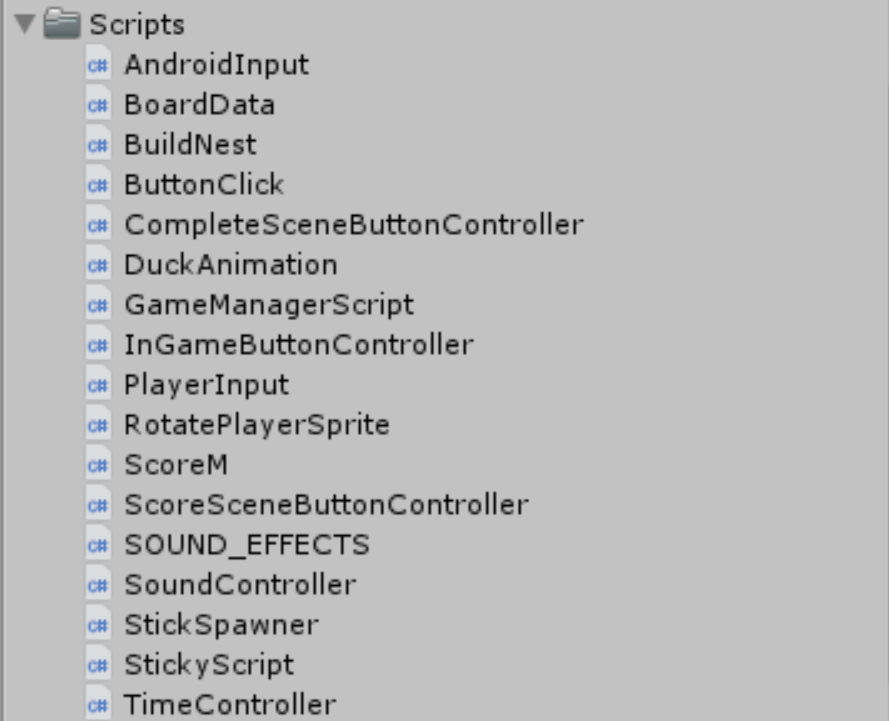
\includegraphics{coderesource.png}
\caption{Code folder structure}
\end{figure}

\subsubsection{AndroidInout}
This script provide function to modify four value of Boolean variables which is used for player control in Android devices. These variables stand for control of:
\begin{itemize}
\item move left.
\item move right.
\item fly up-left.
\item fly up-right.
\end{itemize}
Only when this value is true can the player control the movement in this direction.

\subsubsection{BoardData}
This script provide struck to store the information of player including:
\begin{itemize}
\item name: Player type in the EndScene.
\item score: The time as well as score player spend in gameplay scene.
\end{itemize}
It also provides two functions for sort and debug:
\begin{itemize}
\item CompareTo(Score other): Compara to other Score, return the difference value between them.
\item ToString(): Print the name and the score in console for debug.
\end{itemize}

\subsubsection{BuildNest}
This script is attached to the nest which player intend to build. It provide the function named AdvanceNestStage() that will be called every time the stick brought back and update the image of nest for five levels.

\subsubsection{ButtonClick}
This Script provide function used in button clicked of StartScene.It provides button response as follow:
\begin{itemize}
\item OnLoginButtonClick(): Load the MainScene and start the game.
\item OnExitButtonClick(): Quit the game.
\item OnOptionButtonClick(): Open the option by setting the active of option panel to true.
\item OnBackButtonClick(): There is a button on the option to close the option by setting the active of option panel to false.
\item OnLeaderBoardClick(): Load the score scene and show the leader board to player.
\end{itemize}

\subsubsection{CompleteSceneButtonController}
There is only one function in this script that used in EndScene. When players enter their name in textfield in EndScene and click Apply button, it will store the players name and score into a struct which is built to store player information for leader board and return to StartScene. 

\subsubsection{DuckAnimation}
The main purpose of this script is to control the animation of duck. It will keep tracking the statement of duck to make sure the animation is make sense. This script includes two parts:
\begin{itemize}
\item Uncontrollable check: When the player collide with a owl, it will fall down and lose control for seconds. And there will be a symbol show up above the duck's head, telling player that they cannot control the duck.
\item hastwigs check: When the player has already collected a stick, a stick image will show up on the duck's head.
\end{itemize}

\subsubsection{GameManagerScript}
This Script control some basic function in gameplay scene including:
\begin{itemize}
\item Time record: Record the time that player used in collecting stick. It will reset when the game restart and stop recording when game finished.
\item PickUpSticks(): change the value of hastwig to true, limitating player cannot collect the second stick.
\item AddedStickToNest(): When player bring stick back to the nest, change the value of hastwig to make player available to collect stick again.
\item CanBuild(): Return the value of hastwig to show if the nest is available for building.
\end{itemize}
There is also a function here to print the time that player used to a file for testing.

\subsubsection{InGameButtonController}
The response of button in MainScene is controlled by this script.The functions are list below:
\begin{itemize}
\item Time record: Record the time that player used in collecting stick. It will reset when the game restart and stop recording when game finished.
\item OnPause(): When user click option button on the right-up corner of screen, the option panel will appear and the game will pasue by change the Time.timeScale to 0;
\item OnResume(): When option panel is in the front of scene and game pause, player can click Resume button to back to game.
\item OnRestart(): When option panel is in the front of scene and game pause, player can click Restart button to restart the game by reloading the gameplay scene.
\item OnReturnMenu(): When option panel is in the front of scene and game pause, player can click Return button to back to the StartScene.
\item CloseTutorial(): Close the tutorial in gameplay scene by clicking OK button on the tutorial panel.
\end{itemize}

\subsubsection{PlayerInput}
The functions to distinguish the player's different input and collision that happened in duck is stored in this script. The flight time limitation is 5 seconds, requiring player to touch ground to reset. The player's input will be detected in the following order:
\begin{itemize}
\item Left and fly: When player presses both left and up button, it will call the movement function MoveLeftAndUp() and set the corresponding animation.
\item Right and fly: When player presses both right and up button, it will call the movement function MoveRightAndUp() and set the corresponding animation.
\item Left: When player simply presses left button, it will call the movement function MoveLeft() and set the corresponding animation.
\item Right: When player simply presses right button, it will call the movement function MoveRIght() and set the Corresponding animation.
\item Fly: When player simply presses up button, it will call the movement function Fly() and set the corresponding animation.
\item Not fly: When player dose not press up button, it will call no function and reset the animation of duck. This situation also include pressing nothing.
\end{itemize}

This game also define four types of input when platform is Android, distinguished by divide the screen into 4 parts:
\begin{itemize}
\item TR: Top right.Call the movement function MoveRightAndUp() and set the corresponding animation.
\item TL: Top left.Call the movement function MoveLeftAndUp() and set the corresponding animation.
\item BL: Bottom left.Call the movement function MoveLeft() and set the corresponding animation.
\item BR: Bottom right.Call the movement function MoveRIght() and set the Corresponding animation.
\end{itemize}
The 5 types of movement also placed here:
\begin{itemize}
\item MoveLeftAndUp(): Executing only when flight time is greater than 0, it will give the player a predefined speed and tilt a little bit in the left.
\item MoveRightAndUp(): Executing only when flight time is greater than 0, it will give the player a predefined speed and tilt a little bit in the right.
\item MoveLeft(): It will give the player a predefined speed in the left.
\item MoveRIght(): It will give the player a predefined speed in the right.
\item Fly():Executing only when flight time is greater than 0, it will give the player a predefined speed and tilt a little bit.
\end{itemize}

The responses of collision are also placed in this script:
\begin{itemize}
\item collide with owl: If the player collide with a owl, it will lose control, fall down and lose stick if possible.
\item collide with twiggy: If the player collide with a twig, it will collect it.
\item collide with nest: If the player collide with nest and has a twig, the nest will be built.
\item collide with Respawn: If the player collide with object tagged as Respawn, it will back to nest. Tag of Respawn is attached to hole and under the cliff.
\item collide with Ground: If the plyaer collide with object tagged as Ground, it will get power to fly again by setting the flight time back to 5 seconds. Tag of Ground is attached to tree, mountain, ground and titles.
\end{itemize}

\subsubsection{RotatePlayerSprite}
This script is called mainly when the player is moving to change the duck direction. It rotate the duck by x, y and z which Initialised to 0.
\begin{itemize}
\item SetX(float i): Change x to i.
\item SetY(float i): Change y to i.
\item SetZ(float i): Change z to i.
\item DoRotation(): Rotate according to the incoming parameter x, y and z.
\end{itemize}

\subsubsection{ScoreM}
The main purpose of this script is to manager the score. It has functions as below:
\begin{itemize}
\item showScore(): This function will be call in score scene and show the top 3 information of player to leader board.
\item LoadScore(): This function will be call every time the MainScene is loaded. It will get the informtaion from local file and store them in a array for future work.
\item addScore(string name, int score, List<Score> LS): This function will be called every time that the player click Apply button after they finish the game and type their name. It will add the new information of player to the array.
\item sortScore(): This function will be called every time a scene loaded. It will sort the information of player by their score. It will only store the top 3 and remove the rest.
\end{itemize}

\subsubsection{ScoreSceneButtonController}
This script contains only one function that jump back to StartScene from score scene when player click Back button. 

\subsubsection{SOUNDEFFECTS}
This script is attached to the player to control the sound effect. When the player collide with the owl, it will play the sound effect of fall down.

\subsubsection{SoundController}
This script is attached to canvas to control the volume in game by dragging the slider.

\subsubsection{StickSpawner}
The main purpose of this script is to manager the stick spawned in game. It define 4 basic variables:
\begin{itemize}
\item maxStickCount: Maximum number of branches allowed in the game.
\item lastSpawn: The time between two stick spawned.   
\item DistanceToPlayer(): This function return the distance from one stick to player.
\item Enabled(): This function return if the stick is visible to player.
\end{itemize}
By using the above variables, stick are limited to generating once every 6 seconds, and the number will not exceed 10. The stick will be delete if it is too far away from the player or invisible.

\subsubsection{StickyScript}
This script is used to count the number of stick. It contains two parts:
\begin{itemize}
\item check invisible: If the stick is invisible to player, destroy it and reduce stick count by one.
\item check collection: If the stick is collected by player, destroy it and reduce stick count by one.
\end{itemize}

\subsubsection{TimeController}

This script is to create a timer for the player to observe how long he has spent.

\subsection{Tools used to produce code (tools to build the game)}
The main tools used in this project are list below:
\begin{itemize}
\item Unity3D 2018.1.7f Personal
\item Visual Studio community 2017
\item Adobe Illustrator CC 2015
\item Adobe Photoshop CC 2015
\item Overture 5
\end{itemize}
A game is an application which player can interact with by pressing controller (Keyboard) to give input to system. Then the game engine handles this input, making them available for the script to query. If any change occurs in game, the game engine will send information to renders to reflect the change.
 
\subsubsection{Unity3D}
This project choose unity3D as game engine which offers a primary scripting API in C\#. It integrates many useful packages including Input Manager and provide Unity Collaborate where developers can create game together seamlessly. Collaborate features makes it easy for Unity teams to save, share, and sync their project with others. It’s cloud enabled, built directly into Unity, and has a simplified workflow that is easy to use, regardless of location and discipline. In order to make sure all the group members are free of compilation problem, the developer should use the same version.

\subsubsection{Visual Studio} 
As one of the most popular integrated development environments in the world, Visual Studio has excellent support to Unity3D. It provides Visual Studio Tools for Unity add-on which formerly known as UnityVS to developer. The developers can attach the debugger and start the game by simply changing the debug target.

\subsubsection{Illustrator CC 2015}
Adobe illustrator, often referred to as "AI", is an industrial standard vector illustration software for publishing, multimedia and online images.It is a very excellent vector graphics processing tool.

\subsubsection{Photoshop}
Besides a few resources from Unity3D Assets Store, there are some simple images produced by Photoshop. For instance, tree, mountain and owl.

\subsubsection{Overture}
The background music is produced by ourselves using overture. Creating a simple melody and put the notes in the correct position, Overture can produce a midi or .wav format back ground music.

\section{Testing}
\game{Sticky Beaking}{ } is the final iteration of the initial product from the 2019 Global Game Jam, \game{Cluster Duck}{}.

\subsection{Strategy}
The testing strategy for \game{Stick Beaking}{ } revolved around small testing cycles continually conducted throughout the GGJ weekend (starting 25$^{th}$ January 2019 at 17:00 and ending 27$^{th}$ January 2019 at 17:00). The goal of the GGJ was to produce a playable bug free unique game by Sunday 25$^{th}$ January by 15:00. \game{Cluster Duck}{ } was ready and uploaded just after this soft deadline.

Due to the extremely tight nature of the development time frame, every team member tested their own creations. Semi-frequently (about once hour, unless there was a big update) all members would upload their changes using Unity's inbuilt version control system, Unity Cloud, to sync the different projects to a similar state so that the game could be tested as a whole; not just its constituent parts.

Each time a mechanic was implemented enough to be tested, the developer of the mechanic would test the code by playing the game, seeing if it functioned as expected; if the code malfunctioned it was reworked until working satisfactorily.

Post-GGJ, with the game in a stable mostly working state the game was refined and any outstanding bugs fixed so that development on android could begin.

\subsection{Important Test Results}
\begin{table}[H]
\centering
\begin{tabular}{| p{6cm} | p{1.5cm} | p{6cm} |}
     \hline
     \bf Test & \bf Result & \bf Outcome\\ \hline
     The player can move their token up, left and right by using keyboard `W' for flight, `A' for left and `D' for right. & Success & Player token moves in the direction instructed by user. \\ \hline
     Player token sprite rotates to match direction of travel.& Success & player token rotates to match direction of player's input. \\ \hline
     Player token has a limited flight time, upon it decaying to zero player falls until hitting another token that resets its flight time.& Success & Player is limited to 5 seconds of flight before needed to land and reset the timer.\\ \hline
     Tokens reset player flight time (trees with colliders, the ground and rocks) & Success & Player can reset the flight time by landing on the ground or rock \\ \hline
     When Owl token collides with player token it will become uncontrollable for two seconds& Success & Upon collision with owl tokens player inputs are ignored for two seconds.\\ \hline
     Twigs spawn randomly on the map with a percentage chance each game tick. & Success & Twigs spawn in a radius around the stick spawning game object. \\ \hline
     Player can pick up twigs by colliding with them.& Success & Twig is placed in the duck's mouth. and rotates with the duck sprite.\\ \hline
     While carrying a twig and colliding with nest object, the stick should be removed and the nest advances a build stage.& Success & The stick appears to be deposited on the nest, adding another section to the nest sprite. \\ \hline
     On collision with owls and while carrying a stick, the stick should be destroyed.& Fail & Player can collide with owls and keep the stick. \\ \hline
     Player teleports when falling down into the vorago, losing the stick as a penalty& Fail& Player can use this as a shortcut to return to the nest with stick advancing the game.\\ \hline     
     After losing sticks to owls and voragoes, player should be free to collect another stick.& Untested & Cannot test as player does not lose stick in either of the situations. \\ \hline
     
\end{tabular}
\caption{Tests conducted during the GGJ, showing the result and outcome.}
\label{tab:ggjtestingtable}
\end{table}

\begin{table}[H]
\centering
\begin{tabular}{| p{6cm} | p{1.5cm} | p{6cm} |}
     \hline
     \bf Test & \bf Result & \bf Outcome\\ \hline
     Upon Completion of the nest the game progresses to an ending screen. & Fail & Game does not progress when nest is fully built. Serious re-occurring repeatable issue while running from the executable. \\ \hline
     Stick spawning events are too numerous. & Success & reduced chance of stick spawning chance from over 50\% to almost 0 each game tick. \\ \hline
     Too many trees have colliders so it is too easy to reset flight time. Trees also severely impact fun of the gameplay by being in the way. & Success & Removed excess trees from map. \\ \hline
     Duck Animation (flying)& Success & Duck animation works when player directs the object to move. \\ \hline
     Tutorial is dismissable via button. & Success & Tutorial screen is dismissable, however shows up each time a new game is started. Look at adding a flag to only show it for the first time.\\ \hline
     Progression to ending scene functioning as expected.& Success & Added a check to see if a file and directory were present in folder structure. If not it creates the file allowing the game to move on to the ending scene instead of hanging in main scene.\\ \hline
     On collision with owls and while carrying a stick, the stick should be destroyed.& Success & Upon collision with owls the player now loses the stick, and hasTwig flag in game manager is reset to false. \\ \hline
     Player teleports when falling down into the vorago, losing the stick as a penalty& Success& Player now loses the stick when falling down. No longer abusable.\\ \hline     
     After losing sticks to owls and voragoes, player should be free to collect another stick.& Success & Player is free to pick up the next stick they find without any unintended consequences from losing it previously. \\ \hline
\end{tabular}
\caption{Tests conducted after the GGJ, showing the result and outcome.}
\label{tab:postggjtestingtable}
\end{table}

\begin{table}[H]
\centering
\begin{tabular}{| p{6cm} | p{1.5cm} | p{6cm} |}
     \hline
     \bf Test & \bf Result & \bf Outcome\\ \hline
     Unity Android Build & Success & Game launches and UI behaves as the PC version does.\\ \hline
     Rotating screen rotates game to the correct orientation. & Success & Game restarts in the correct orientation.\\ \hline
     Pressing in the top left of the screen (regardless of orientation) will make the player token fly left. & Success & Pressing in this quadrant the player will fly left. \\ \hline
     Pressing in the top right of the screen (regardless of orientation) will make the player token fly right & Success & Press in this quadrant makes the player fly right.\\ \hline
     Pressing in bottom left of screen (regardless of orientation) will make the player token move left (not fly)  & Fail & Unresponsive. \\ \hline
     Pressing in bottom right of screen (regardless of orientation) will make the player token move right (not fly)  & Fail & Unresponsive. \\ \hline
     Fly left button depressed causes player token to move vertically and horizontally left. & Fail & Unresponsive. \\ \hline
     Fly right button depressed causes player token to vertically and horizontally right. & Fail & Unresponsive. \\ \hline
     Left button depressed causes player token to move horizontally left. & Fail & Unresponsive. \\ \hline
     Right button depressed causes player token to move horizontally right. & Fail & Unresponsive. \\ \hline
     
\end{tabular}
\caption{Tests conducted after the GGJ for Android, showing the result and outcome.}
\label{tab:androidtestingtable}
\end{table}

\subsection{Testing for Android Devices}
Testing android devices proved a tricky. All machines used by the team had the Android SDK as well as Android Studio and JDK installed. However even with all the prerequisites completed, successful building of an Android application package would only successfully complete on one machine with the other three machines arguing that the Android SDK was not installed. 

As 3 out of 4 team members were programming for Android blind, and only having one person able to test any code written for that platform made development tricky. Ultimately leading to the incompleteness of \game{Sticky Beaking}{ } for Android.

\section{Feedback from Players}
As we have done marketing for the game and collected feedback from the players to analyse the value of the product we developed. For collecting feedback we have created a link of the game to download it, which is attached to the feedback form.

As a result we got approx 50percent of users like the game and more then 50 percent suggested this game for kids to play. Approximately 25 percent of user played well and got high score range. 

\begin{figure}[H]
\centering
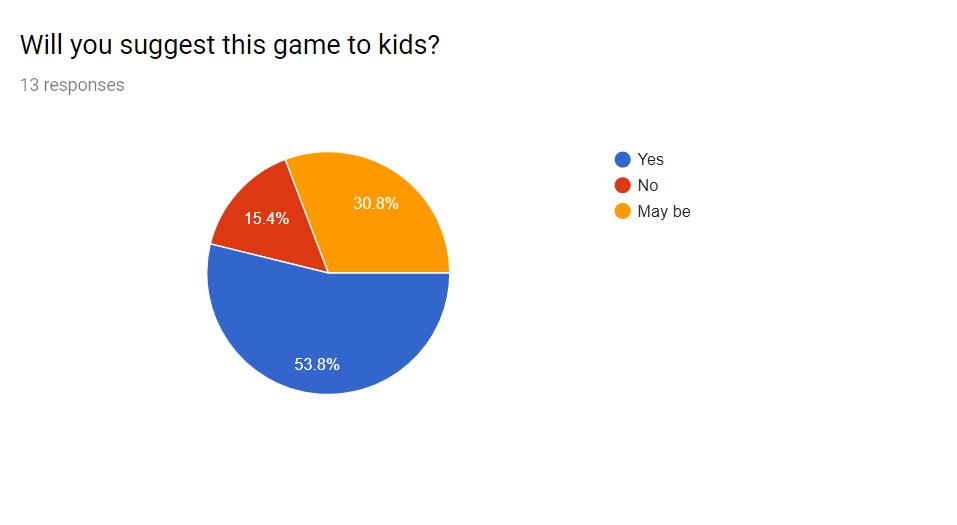
\includegraphics[scale=0.7]{e.png}
\caption{Pie chart representation for the question "Will you suggest this game to kids?" }
\label{suggestiontokids}
\end{figure}

\begin{figure}[H]
\centering
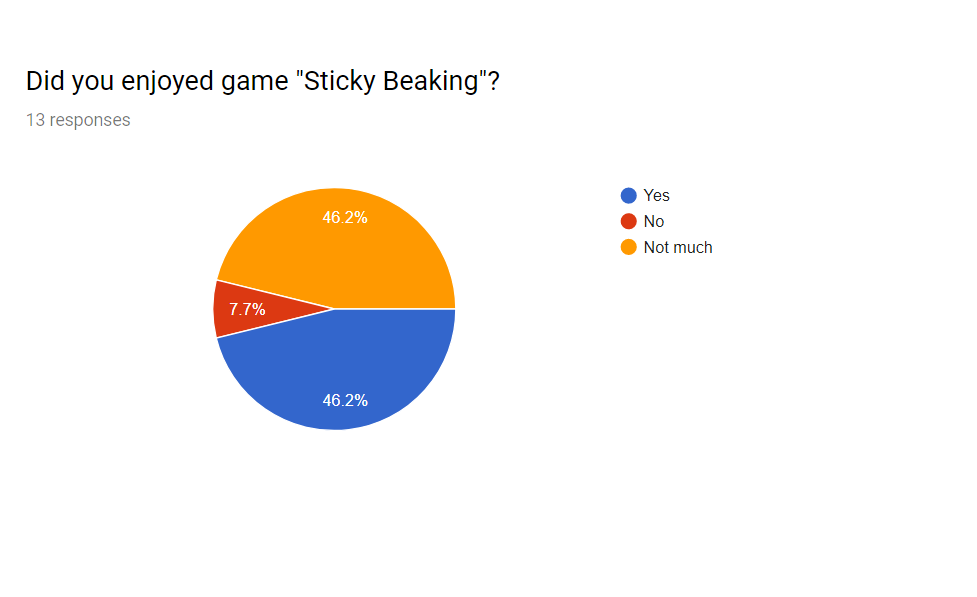
\includegraphics[scale=0.7]{f.png}
\caption{Pie chart representation for the question "Did you enjoyed game Sticky Beaking ?" }
\label{enjoyed}
\end{figure}

\begin{figure}[H]
\centering
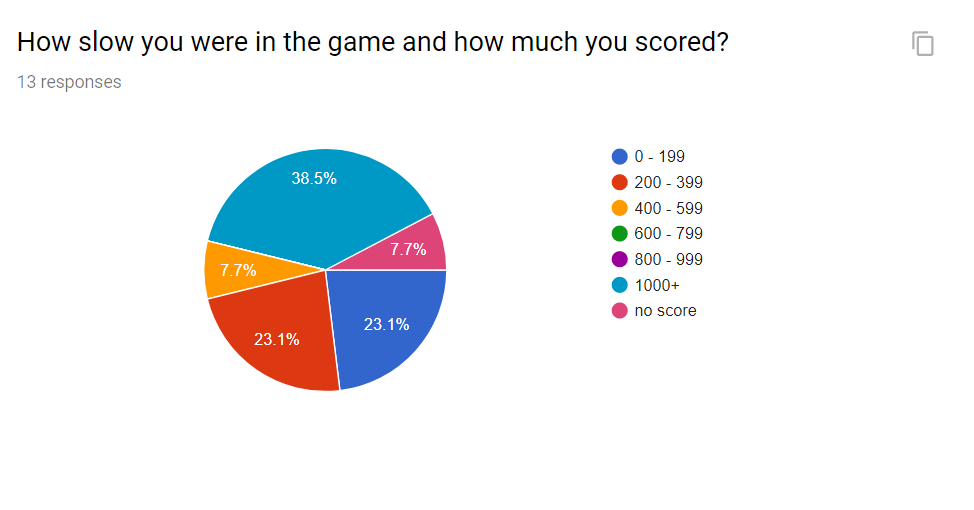
\includegraphics [scale=0.7]{w.png}
\caption{Pie chart representation for the question "How slow you were in the game and how much you scored?" }
\label{score}
\end{figure}

\begin{figure}[H]
    \centering
    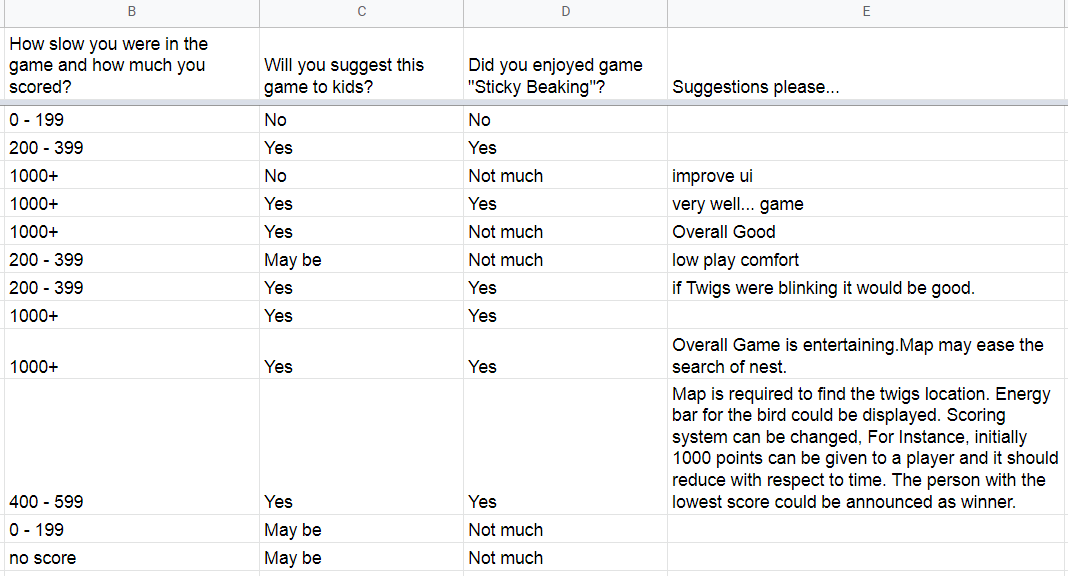
\includegraphics [scale=0.7]{feedback_table.png}
    \caption{Feedback table for the game "Sticky Beaking"}
    \label{feedback}
\end{figure}


\section{Conclusions}
\subsection{System}
The basic functions of this project have been completed, Including:
\begin{itemize}
\item Playable character with time limitation in fly.
\item Collectable items to build the nest.
\item Nest with 7 levels to make game finished.
\item time calculated as player score.
\item leaderboard to show the rank of players.
\end{itemize}
There are something can be extend in the future:
\begin{itemize}
\item Online leaderboard: Build a server to store score from all players in different platforms.
\item More scene : There is only one playable scene now, it can have more levels for different difficulty. 
\item Android version: A mobile version for players can play the game wherever they are.
\end{itemize}

\subsection{Evaluation of tools and language}
Unity3D is the preferred 3D engine for most game development teams nowadays, and its performance on 2D is also excellent. It can easily solve many problems that other engines cannot.
\begin{itemize}
\item Integrated IDE environment: It is very convenient to edit the components in the game. For example, animation editing can be done directly in the editor.
\item Component-based object system: Each object in the game has its own components, which is convenient for development.
\item Real-time: Game can be compiled and preview before building. Developer even can change parameter during play mode which help to develop new function faster.
\item Unity3D Assets Store: Unity3D provide Assets Store which have many resource that developers can refer to.
\end{itemize}
Visual Studio has a excellent support to Unity3D code work. For instance, every time you restart the project, the Visual Studio will automatically locate where you left last time. It automatically debug function is also excellent by support of Unity3D package. These greatly improve the efficiency of the program.


\subsection{Project management}

The following figure will provide work breakdown structure and Gantt chart to show the management for the  project. The main sub-tasks and the relationship between them can be known in breakdown structure. In the work breakdown structure, the whole project is divided into 2 parts. In Gantt chart, a complete and detailed timetable is given.

\begin{figure}[H]
    \centering
    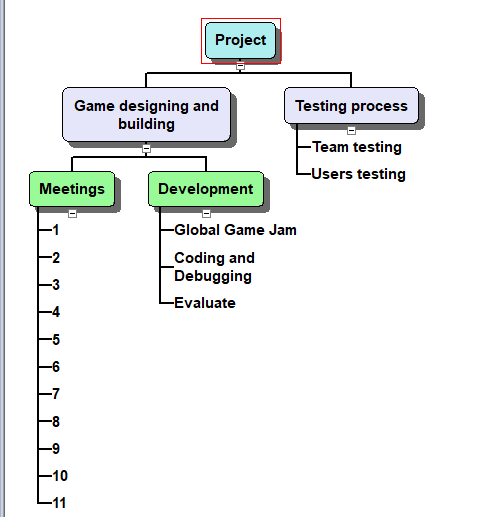
\includegraphics{images/WBS.png}
    \caption{Work breakdown structure}
    \label{fig:wbs}
\end{figure}

\newpage

    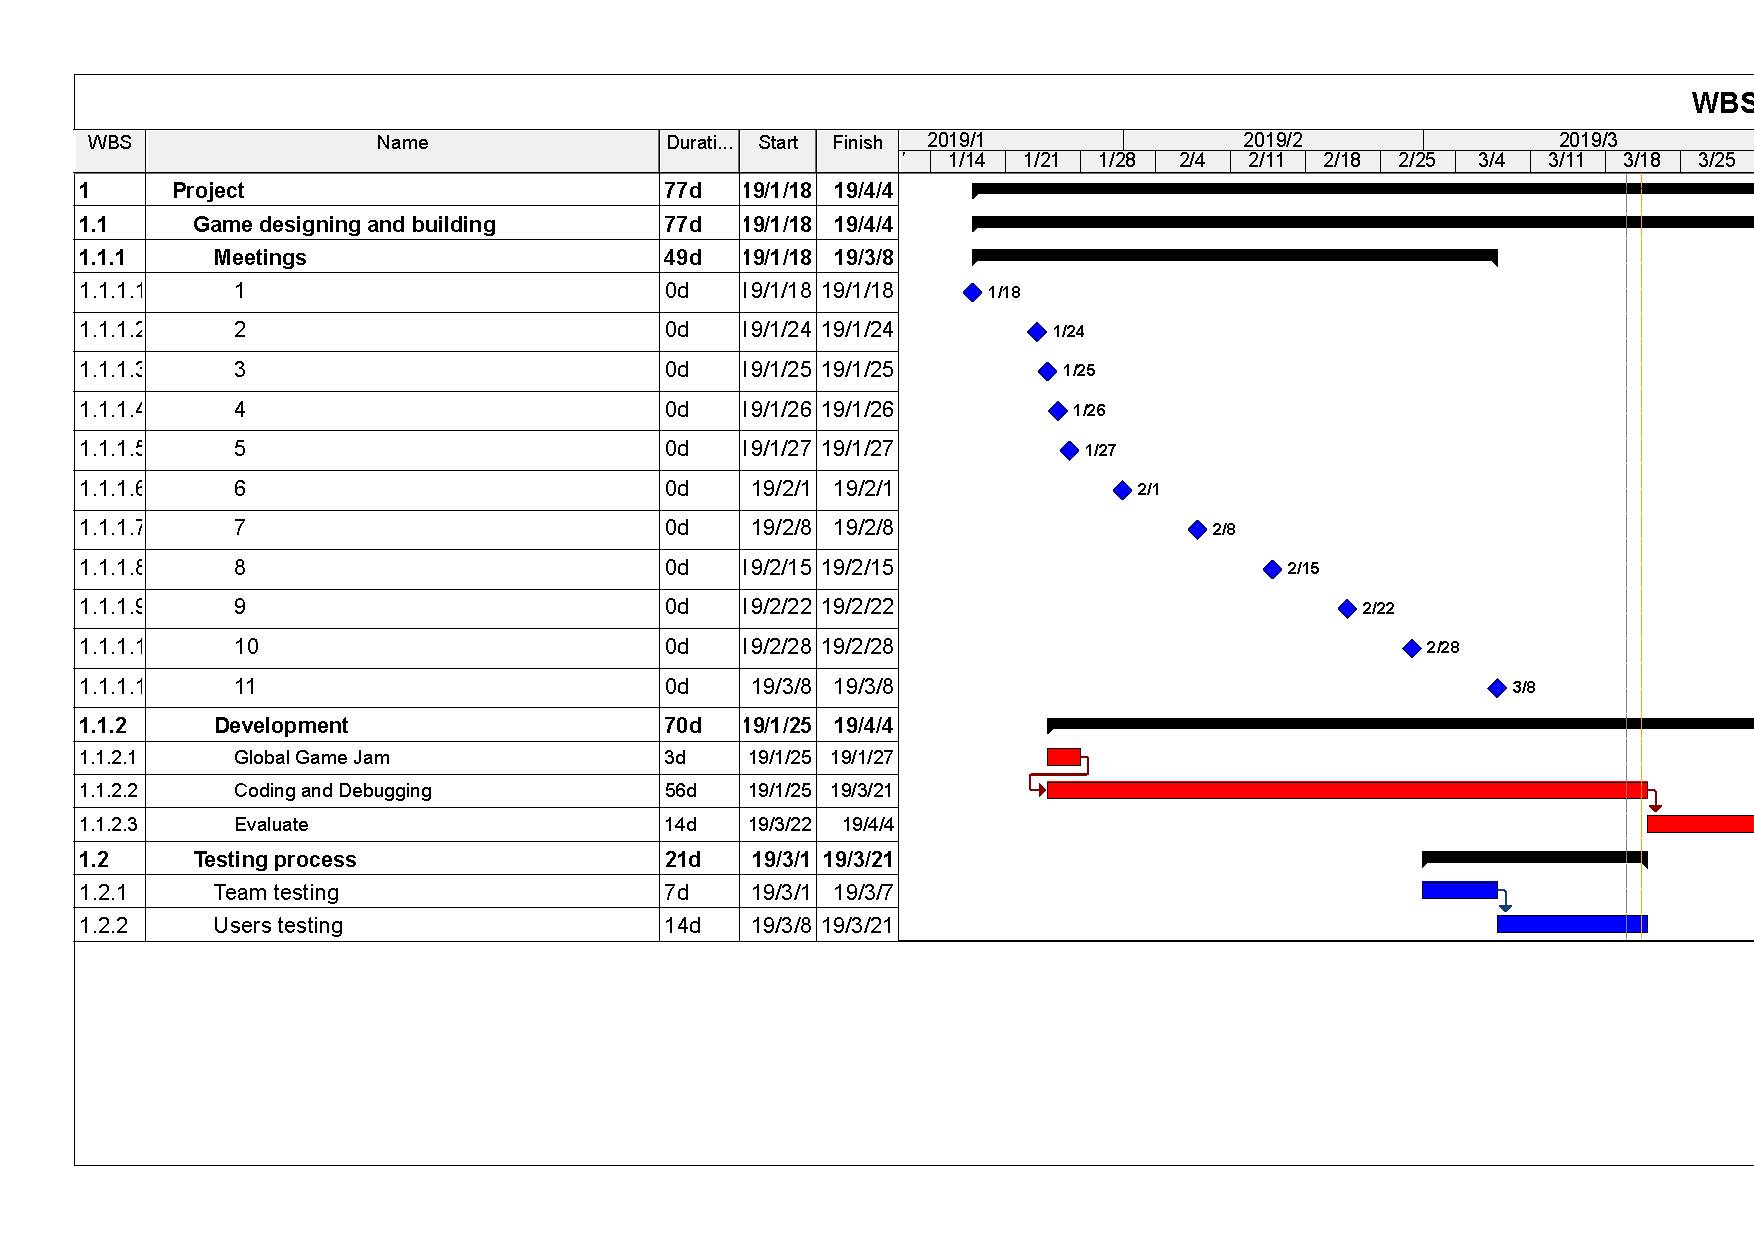
\includepdf[pages=1-2,landscape=true]{images/Gantt}



%leave everything below this comment the way it is.
\newpage
\bibliographystyle{IEEEtran}
\bibliography{./references}

\end{document}